\documentclass{article}
\usepackage{graphicx, tikz-cd, float, titlepic, booktabs} % Required for inserting images
\usepackage{amsmath, amssymb, amsthm, amsfonts, siunitx, physics, gensymb}
\AtBeginDocument{\RenewCommandCopy\qty\SI}
\usepackage[version=4]{mhchem}
\usepackage[most,many,breakable]{tcolorbox}
\usepackage{xcolor, fancyhdr, varwidth}
\usepackage[Glenn]{fncychap}
%Options: Sonny, Lenny, Glenn, Conny, Rejne, Bjarne, Bjornstrup
\usepackage{hyperref, cleveref}
\usepackage{icomma, enumitem} %comma as decimal and continue enumerate with [resume]
\usepackage[danish]{babel}
%%%%%%%%%%%%%%%%%%%%%%%%%%%%%%
% SELF MADE COLORS
%%%%%%%%%%%%%%%%%%%%%%%%%%%%%%
\definecolor{myg}{RGB}{56, 140, 70}
\definecolor{myb}{RGB}{45, 111, 177}
\definecolor{myr}{RGB}{199, 68, 64}
\definecolor{mytheorembg}{HTML}{F2F2F9}
\definecolor{mytheoremfr}{HTML}{00007B}
\definecolor{mylenmabg}{HTML}{FFFAF8}
\definecolor{mylenmafr}{HTML}{983b0f}
\definecolor{mypropbg}{HTML}{f2fbfc}
\definecolor{mypropfr}{HTML}{191971}
\definecolor{myexamplebg}{HTML}{F2FBF8}
\definecolor{myexamplefr}{HTML}{88D6D1}
\definecolor{myexampleti}{HTML}{2A7F7F}
\definecolor{mydefinitbg}{HTML}{E5E5FF}
\definecolor{mydefinitfr}{HTML}{3F3FA3}
\definecolor{notesgreen}{RGB}{0,162,0}
\definecolor{myp}{RGB}{197, 92, 212}
\definecolor{mygr}{HTML}{2C3338}
\definecolor{myred}{RGB}{127,0,0}
\definecolor{myyellow}{RGB}{169,121,69}
\definecolor{myexercisebg}{HTML}{F2FBF8}
\definecolor{myexercisefg}{HTML}{88D6D1}
%%%%%%%%%%%%%%%%%%%%%%%%%%%%%%%%%%%%%%%%%%%%%%%%%%%%%%%%%%%%%%%%%%%%%%
% Box environments for theorems and problems
%%%%%%%%%%%%%%%%%%%%%%%%%%%%%%%%%%%%%%%%%%%%%%%%%%%%%%%%%%%%%%%%%%%%%
\setlength{\parindent}{1cm}
%================================
% Question BOX
%================================
\makeatletter
\newtcbtheorem{question}{Opgave}{enhanced,
	breakable,
	colback=white,
	colframe=myb!80!black,
	attach boxed title to top left={yshift*=-\tcboxedtitleheight},
	fonttitle=\bfseries,
	title={#2},
	boxed title size=title,
	boxed title style={%
			sharp corners,
			rounded corners=northwest,
			colback=tcbcolframe,
			boxrule=0pt,
		},
	underlay boxed title={%
			\path[fill=tcbcolframe] (title.south west)--(title.south east)
			to[out=0, in=180] ([xshift=5mm]title.east)--
			(title.center-|frame.east)
			[rounded corners=\kvtcb@arc] |-
			(frame.north) -| cycle;
		},
	#1
}{def}
\makeatother
%================================
% DEFINITION BOX
%================================

\newtcbtheorem[]{Definition}{Definition}{enhanced,
	before skip=2mm,after skip=2mm, colback=red!5,colframe=red!80!black,boxrule=0.5mm,
	attach boxed title to top left={xshift=1cm,yshift*=1mm-\tcboxedtitleheight}, varwidth boxed title*=-3cm,
	boxed title style={frame code={
					\path[fill=tcbcolback]
					([yshift=-1mm,xshift=-1mm]frame.north west)
					arc[start angle=0,end angle=180,radius=1mm]
					([yshift=-1mm,xshift=1mm]frame.north east)
					arc[start angle=180,end angle=0,radius=1mm];
					\path[left color=tcbcolback!60!black,right color=tcbcolback!60!black,
						middle color=tcbcolback!80!black]
					([xshift=-2mm]frame.north west) -- ([xshift=2mm]frame.north east)
					[rounded corners=1mm]-- ([xshift=1mm,yshift=-1mm]frame.north east)
					-- (frame.south east) -- (frame.south west)
					-- ([xshift=-1mm,yshift=-1mm]frame.north west)
					[sharp corners]-- cycle;
				},interior engine=empty,
		},
	fonttitle=\bfseries,
	title={#2},#1}{def}
\newtcbtheorem[]{definition}{Definition}{enhanced,
	before skip=2mm,after skip=2mm, colback=red!5,colframe=red!80!black,boxrule=0.5mm,
	attach boxed title to top left={xshift=1cm,yshift*=1mm-\tcboxedtitleheight}, varwidth boxed title*=-3cm,
	boxed title style={frame code={
					\path[fill=tcbcolback]
					([yshift=-1mm,xshift=-1mm]frame.north west)
					arc[start angle=0,end angle=180,radius=1mm]
					([yshift=-1mm,xshift=1mm]frame.north east)
					arc[start angle=180,end angle=0,radius=1mm];
					\path[left color=tcbcolback!60!black,right color=tcbcolback!60!black,
						middle color=tcbcolback!80!black]
					([xshift=-2mm]frame.north west) -- ([xshift=2mm]frame.north east)
					[rounded corners=1mm]-- ([xshift=1mm,yshift=-1mm]frame.north east)
					-- (frame.south east) -- (frame.south west)
					-- ([xshift=-1mm,yshift=-1mm]frame.north west)
					[sharp corners]-- cycle;
				},interior engine=empty,
		},
	fonttitle=\bfseries,
	title={#2},#1}{def}

\newtcbtheorem{theo}%
    {Theorem}{}{theorem}
\newtcolorbox{prob}[1]{colback=red!5!white,colframe=red!50!black,fonttitle=\bfseries,title={#1}}
%================================
% NOTE BOX
%================================

\usetikzlibrary{arrows,calc,shadows.blur}
\tcbuselibrary{skins}
\newtcolorbox{note}[1][]{%
	enhanced jigsaw,
	colback=gray!20!white,%
	colframe=gray!80!black,
	size=small,
	boxrule=1pt,
	title=\textbf{Note:},
	halign title=flush center,
	coltitle=black,
	breakable,
	drop shadow=black!50!white,
	attach boxed title to top left={xshift=1cm,yshift=-\tcboxedtitleheight/2,yshifttext=-\tcboxedtitleheight/2},
	minipage boxed title=1.5cm,
	boxed title style={%
			colback=white,
			size=fbox,
			boxrule=1pt,
			boxsep=2pt,
			underlay={%
					\coordinate (dotA) at ($(interior.west) + (-0.5pt,0)$);
					\coordinate (dotB) at ($(interior.east) + (0.5pt,0)$);
					\begin{scope}
						\clip (interior.north west) rectangle ([xshift=3ex]interior.east);
						\filldraw [white, blur shadow={shadow opacity=60, shadow yshift=-.75ex}, rounded corners=2pt] (interior.north west) rectangle (interior.south east);
					\end{scope}
					\begin{scope}[gray!80!black]
						\fill (dotA) circle (2pt);
						\fill (dotB) circle (2pt);
					\end{scope}
				},
		},
	#1,
}

%%%%%%%%%%%%%%%%%%%%%%%%%%%%%%%%%%%%%%%%%%%%%%%%%%%%%%%%%%%%%%%%%
% SELF MADE COMMANDS
%%%%%%%%%%%%%%%%%%%%%%%%%%%%%%
\newcommand{\sol}{\setlength{\parindent}{0cm}\textbf{\textit{Løsning:}}\setlength{\parindent}{1cm}}
%%%%%%%%%%%%%%%%%%%%%%%%%%%%%%%%%
\usepackage[tmargin=2cm,rmargin=1in,lmargin=1in,margin=0.85in,bmargin=2cm,footskip=.2in]{geometry}\pagestyle{fancy}
\lhead{Minrui Kevin Zhou 2.b}
\rhead{Matematikaflevering 22}

\title{Aflevering 22\\
{\Large \textbf{2.b mat A}}}
\author{Kevin Zhou}
\date{Januar 2024}

\begin{document}
\maketitle
\section*{Bedømmelseskriterier:}
\begin{itemize}
    \setlength\itemsep{3cm}
    \Large
    \item  Redegørelse og dokumentation for metode
    \item Figurer, grafer og andre illustrationer
    \item Notation og layout
    \item Formidling og forklaring
\end{itemize}
\pagebreak
\begin{question}{}{}
  Funktionen $f:[0;2\pi[ \to \mathbb{R}$ er givet ved
\[
  f(x)= \cos(x)
\] 
\begin{itemize}
  \item[a.] Tegn grafen for $f$.
  \item[b.] Løs ligningen
  \[
  \cos(x)=\frac{1}{2}, \quad 0\leq x < 2\pi
  \] 
\end{itemize}
\end{question}
\sol \\ 
\textbf{a.}
Grafen for $f$ kan ses i \cref{fig:cos}. 
\begin{figure}[H]
\begin{center}
  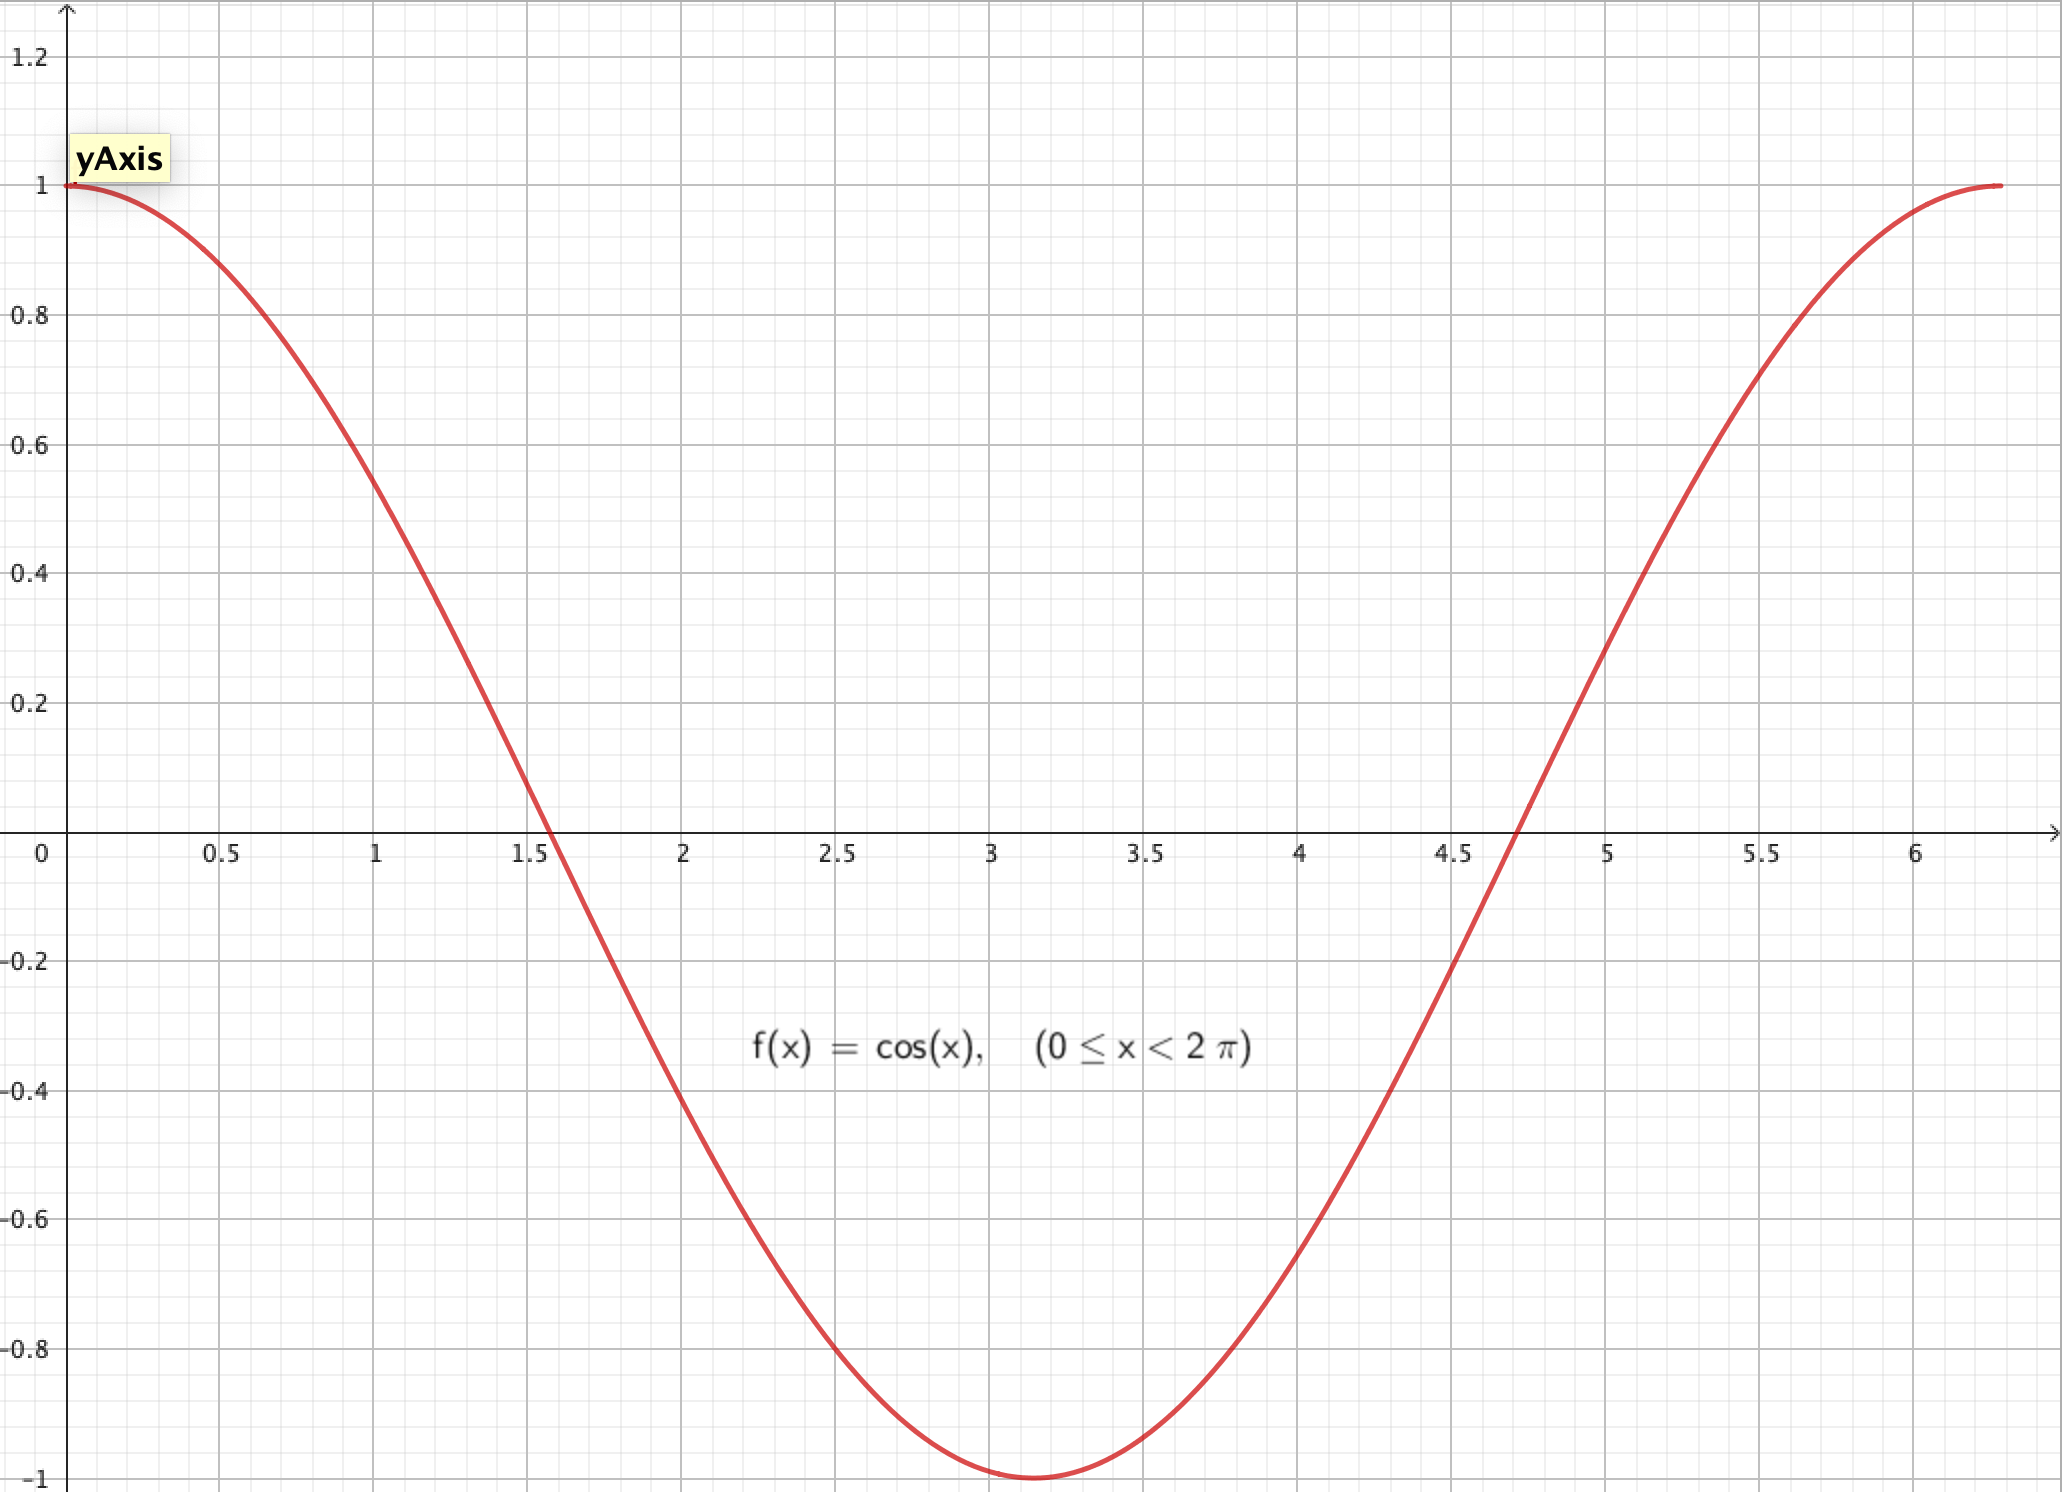
\includegraphics[width=\textwidth]{graf1.png}
\end{center}
\caption{Graf for $f$ tegnet i GeoGebra }
\label{fig:cos}
\end{figure}
\noindent \textbf{b.} Vi løser ligningen.
\begin{equation*}
\begin{split}
  \cos(x)=\frac{1}{2} \land 0\leq x < 2\pi \iff x=\cos^{-1}\left(\frac{1}{2}\right) = \frac{\pi}{3}
\end{split}
\end{equation*}
Læg mærke til, at der kun er en løsning til ligningen, siden afstanden til næste positive løsning til $\cos(x)=\frac{1}{2}$ er $2\pi$.
\begin{question}{}{}
  Funktionen $f:[0;\frac{2\pi}{3}[$ er givet ved
  \[
  f(x)= \sin \left(3x-\pi\right) 
  \] 
  \begin{itemize}
  \item[a.] Tegn grafen for $f$.
  \item[b.] Løs ligningen
  \[
  \sin \left(3x-\pi\right) =-1, \quad 0\leq x < \frac{2\pi}{3}.
  \] 
  \end{itemize}
\end{question}
\sol \\ 
\textbf{a.} Grafen for $f$ ses i \cref{fig:sin}.
\begin{figure}[H]
\begin{center}
  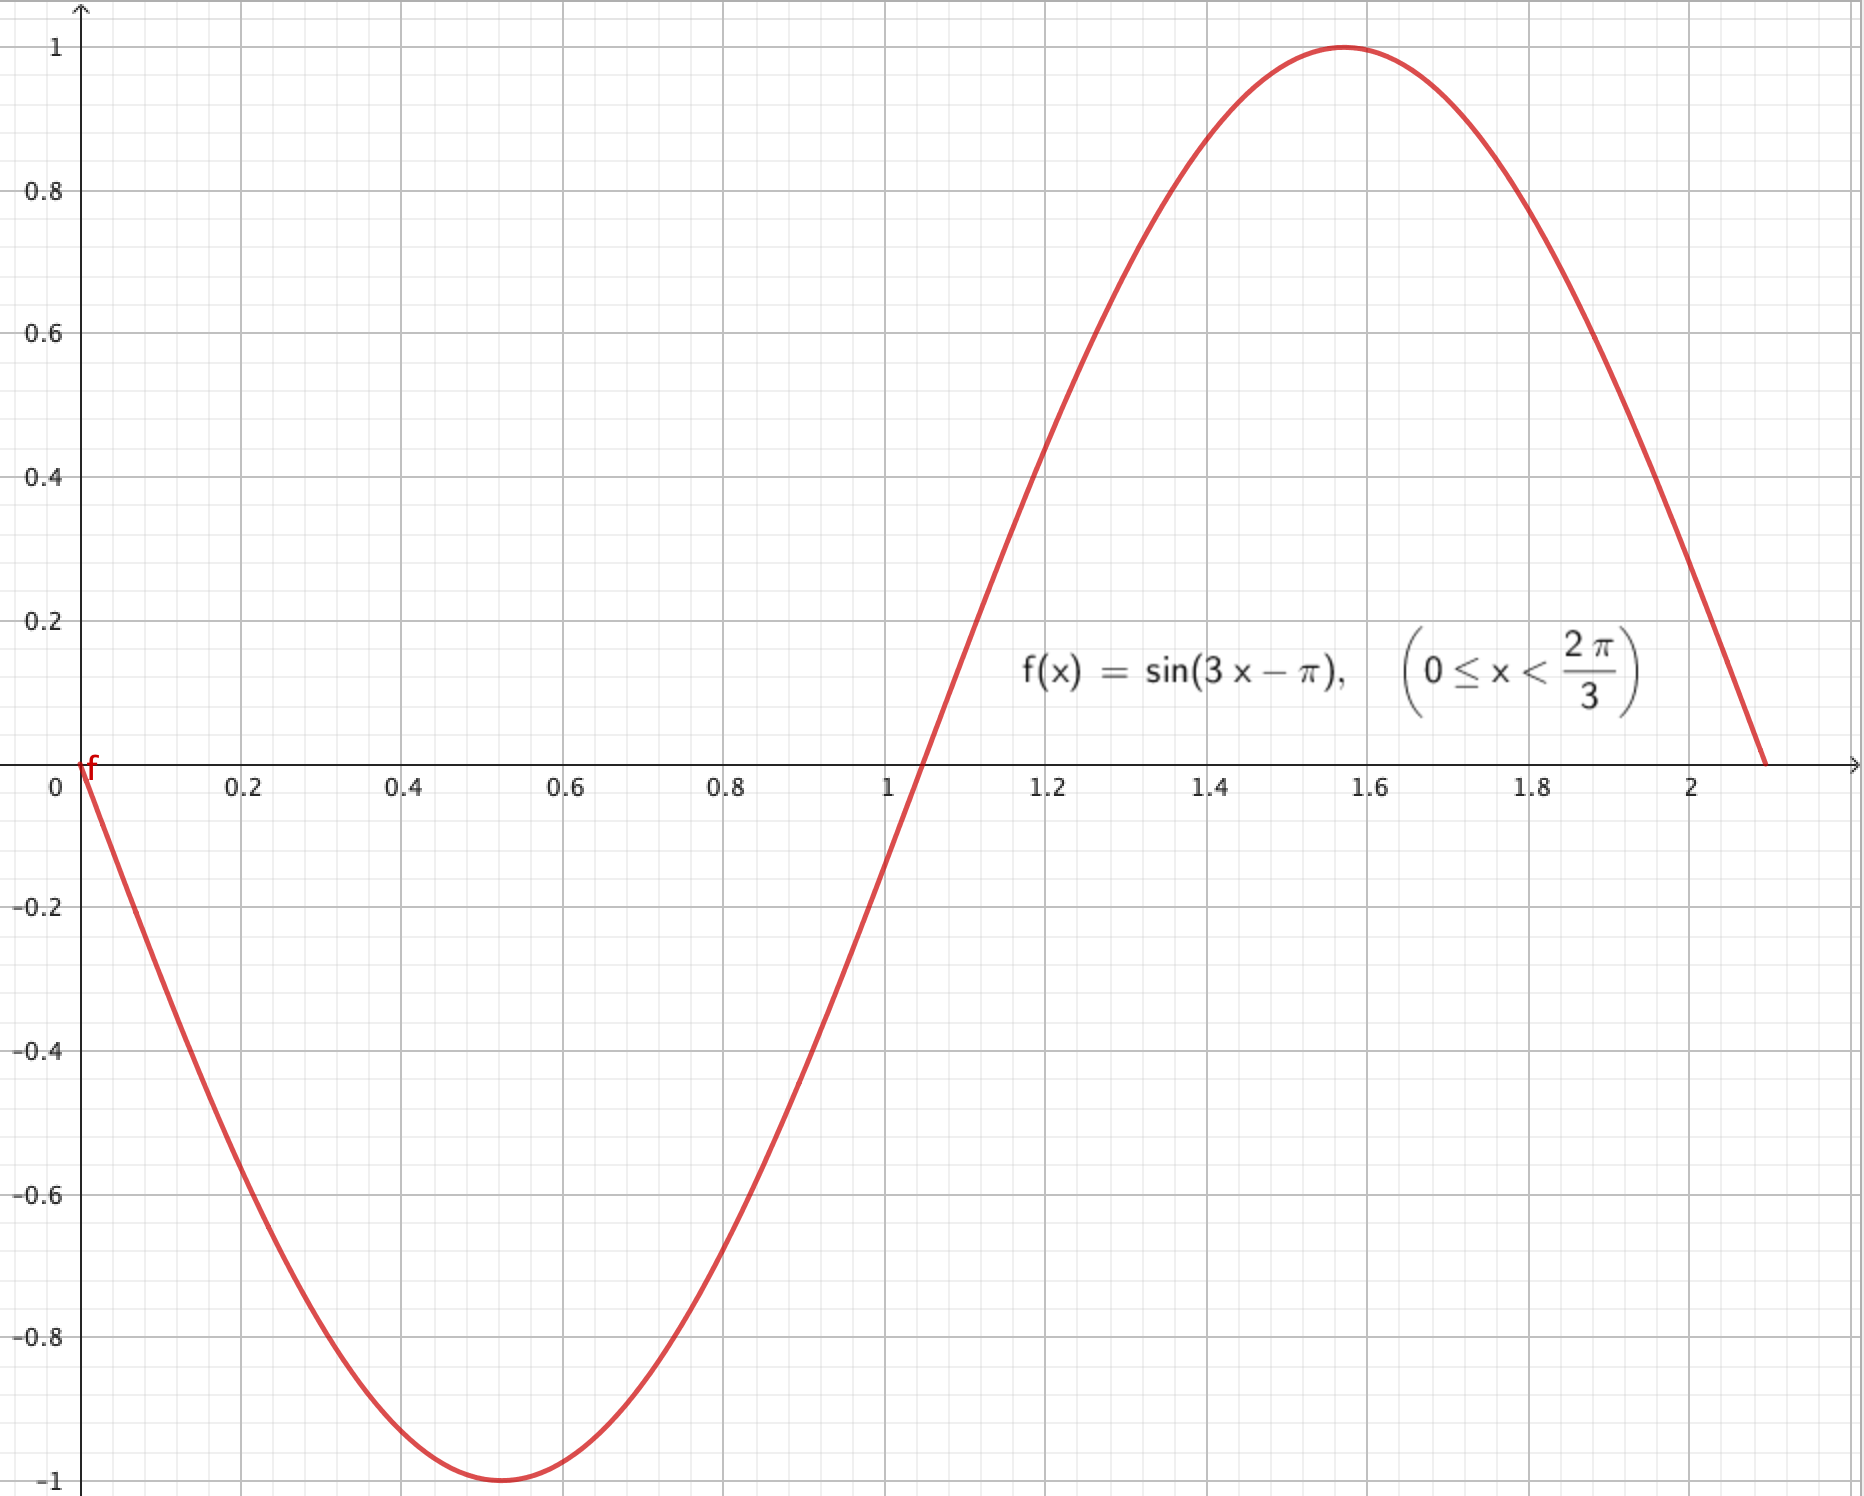
\includegraphics[width=\textwidth]{graf2.png}
\end{center}
\caption{Grafen for $f$ tegnet i GeoGebra }
\label{fig:sin}
\end{figure}
\noindent \textbf{b.} 
Siden der for en funktion af formen $f(t)= A\cdot \sin \left(\alpha t+\varphi\right)+d$ gælder, at den har en periode på $\frac{2\pi}{\alpha}$, så må der gælde, at funktionen $f$ har en periode på $\frac{2\pi}{3}$. 
Derfor har ligningen kun én løsning.
\begin{equation*}
\begin{split}
  \sin \left(3x-\pi\right) =-1\land 0\leq x < \frac{2\pi}{3} &\implies 3x-\pi=-\frac{\pi}{2}\\ 
  &\iff x=\frac{\pi}{6}
\end{split}
\end{equation*}
\begin{question}{}{}
  I en model kan befolkningsudviklingen i Kina beskrives ved
$$
N(t)=\frac{2,2}{1+1,09 \cdot 0,9636^t},
$$
hvor $N(t)$ betegner befolkningstallet i Kina (målt i mia.) til tidspunktet $t$ (målt i år efter 1985). Statistikere har fundet belæg for, at modellen kan bruges til fremskrivning af befolkningstallet i Kina.
\begin{itemize}
  \item[a.] Bestem befolkningstallet til tidspunktet $t=30$.
  \item[b.] Benyt modellen til at bestemme det årstal, hvor befolkningstallet er 1,8 mia.
  \item[c.] Bestem $N^{\prime}(50)$, og forklar betydningen af tallet.
\end{itemize} 
\end{question}
\sol \\ 
\textbf{a.} Vi tager da funktionen $N$ af $30$.
\[
N(30)=\frac{2,2}{1+1,09 \cdot 0,9636^{30}} \approx 1,0730
\] 
Ifølge modellen er befolkningstallet i Kina til tidspunktet $t=30$ altså $1,0730$ mia. \\[1ex]
\textbf{b.} Når befolkningstallet ifølge modellen er 1,8 mia., da gælder der, at
\begin{equation*}
\begin{split}
  \frac{2,2}{1+1,09 \cdot 0,9636^t}=1,8 &\iff 2,2=1,8\cdot \left(1+1,09\cdot 0,9636^t\right) \\ 
  &\implies t=\log_{0,9636}\left(\frac{2,2-1,8}{1,8\cdot 1,09}\right) \approx 42,89
\end{split}
\end{equation*}
Vi runder da op, og årstallet 43 år efter 1985 er 2028.
Altså er årstallet, hvor befolkningstallet er 1,8 mia ifølge modellen 2028. \\[1ex]
\textbf{c.} Vi finder den afledede funktion for $N$ med kædereglen. 
\begin{equation*}
\begin{split}
  N'(t)&=2,2\cdot \left(-\frac{1}{\left(1+1,09\cdot 0,9636^t\right)^2}\right) \cdot 1,09 \cdot 0,9636^t\cdot \ln\left(0,9636\right) \\ 
  &=\left(-\frac{2,398}{\left(1+1,09\cdot 0,9636^t\right)^2}\right) \cdot 0,9636^t\cdot \ln\left(0,9636\right) 
\end{split}
\end{equation*}
Vi tager den afledede funktion af 50.
\begin{equation*}
\begin{split}
  N'(50)&=\left(-\frac{2,398}{\left(1+1,09\cdot 0,9636^{50}\right)^2}\right) \cdot 0,9636^{50}\cdot \ln\left(0,9636\right) \\ 
  &\approx 0,01016
\end{split}
\end{equation*}
Det vil altså sige, at der til tidspunktet $t=50$, hvor årstallet er 2015, så vokser befolkningstallet i Kina ifølge modellen med 0,01016 mia indbyggere per år. 
Det svarer til 10,16 mio indbyggere per år.
\begin{question}{}{}
  I en model kan længden af dagen i Anchorage Alaska som funktion af tiden beskrives ved
  $$
  f(t)=6,61 \cdot \sin (0,0167 t-1,303)+12,2, \quad 0 \leq t \leq 365,
  $$
  hvor $f(t)$ er længden af dagen (målt i timer) til tidspunktet $t$ (målt i døgn efter 1. januar 2011).
  \begin{itemize}
    \item[a.] Benyt modellen til at bestemme længden af dagen i Anchorage Alaska til tidspunktet $t=100$.
    \item[b.] Benyt modellen til at bestemme det tidspunkt, hvor længden af dagen i Anchorage Alaska er størst.
    \item[c.] Bestem $f^{\prime}(100)$, og gør rede for, hvad dette tal fortæller.
  \end{itemize}
\end{question}
\sol \\ 
\textbf{a.} Vi tager da funktionen $f$ af 100.
\begin{equation*}
\begin{split}
  f(100)&= 6,61 \cdot \sin (0,0167 \cdot 100-1,303)+12,2 \\
  &=6,61\cdot \sin \left(0,367\right) +12,2\\ 
  &\approx 14,57
\end{split}
\end{equation*}
Længden af dagen til tidspunktet $t=100$ er ifølge modellen 14,57 timer. \\[1ex]
\textbf{b.} Længden af dagen må være størst når $\sin (0,0167 t-1,303)$ er størst, siden leddet, det indgår i skal være størst muligt for at længden af dagen er størst.
Siden $Vm(\sin)=[-1;1]$, så må der gælde, at længden af dagen er størst når 
\begin{equation*}
\begin{split}
  \sin (0,0167 t-1,303)=1 \land 0\leq t \leq 365 &\implies 0,0167 t -1,303 =\frac{1}{2}\pi \\
  &\implies t=\frac{\frac{1}{2}\pi+1,303}{0,0167}\approx 172
\end{split}
\end{equation*}
Altså er længden af dagen i Anchorage Alaska ifølge modellen størst til tidspunktet $t=172$, der er 172 døgn efter 1. januar 2011.\\[1ex]
\textbf{c.} Vi finder den afledede funktion for $f$ med kædereglen. 
\begin{equation*}
\begin{split}
  f'(t)&=6,61\cdot \cos(0,0167t-1,303)\cdot 0,0167 \\ 
  &= 0,110387 \cdot \cos(0,0167t-1,303)
\end{split}
\end{equation*}
Vi tager den afledede funktion for $f$ af 100.
\begin{equation*}
\begin{split}
  f'(100)&=0,110387 \cdot \cos(0,367) \\ 
  &\approx 0,1030
\end{split}
\end{equation*}
Dette tal fortæller, at dagens længde til tidspunktet $t=100$ vokser med 0,1030 timer per dag. 
\end{document}
